
Further injection tests have been conducted in real data.
The figures in Chapter~\ref{chap6} illustrate the efficiency by which TwoSpect recovers simulated stars in a 0.1 Hz band starting at 142.0 Hz in S6 data.
Additional injection tests, here, show bands with starting frequencies of 162.0 and 222.0 Hz.
In each band, 500 injections were introduced into S6 data; the injection parameters were identical, aside from physically-expected corrections for location and orientation, between the two LIGO interferometers (H1 and L1).
The injection was made and TwoSpect analyzed the entire stretch of S6 (2009 July 09 to 2010 October 20), approximately $4 \times 10^7$ seconds of data, with gaps in the duty cycle of the observatories.
These gaps, arising from trains, logging, wind, earthquakes and other factors disrupting the interferometers, have been a concern, and we wished in part to demonstrate TwoSpect's robustness against them.

%\subsection{Real S6 data: p-weighted $h_0$ recovered vs injected at 142 Hz}
%\begin{figure}
%\caption{\protect\includegraphics[width=0.5\paperwidth,height=0.35\paperheight]{plots/p-weighted/h0UL-vs-h0injected-162-0Hz.eps}}
%Raw $h_0$, and tentative 95\% confidence UL, for 500 injections into\\
%S6 data at 142 Hz (injections also done at 162, 222 Hz)
%\end{figure}

\section{Real S6 data: detection efficiency at 162 Hz}

\begin{figure}
\begin{center}
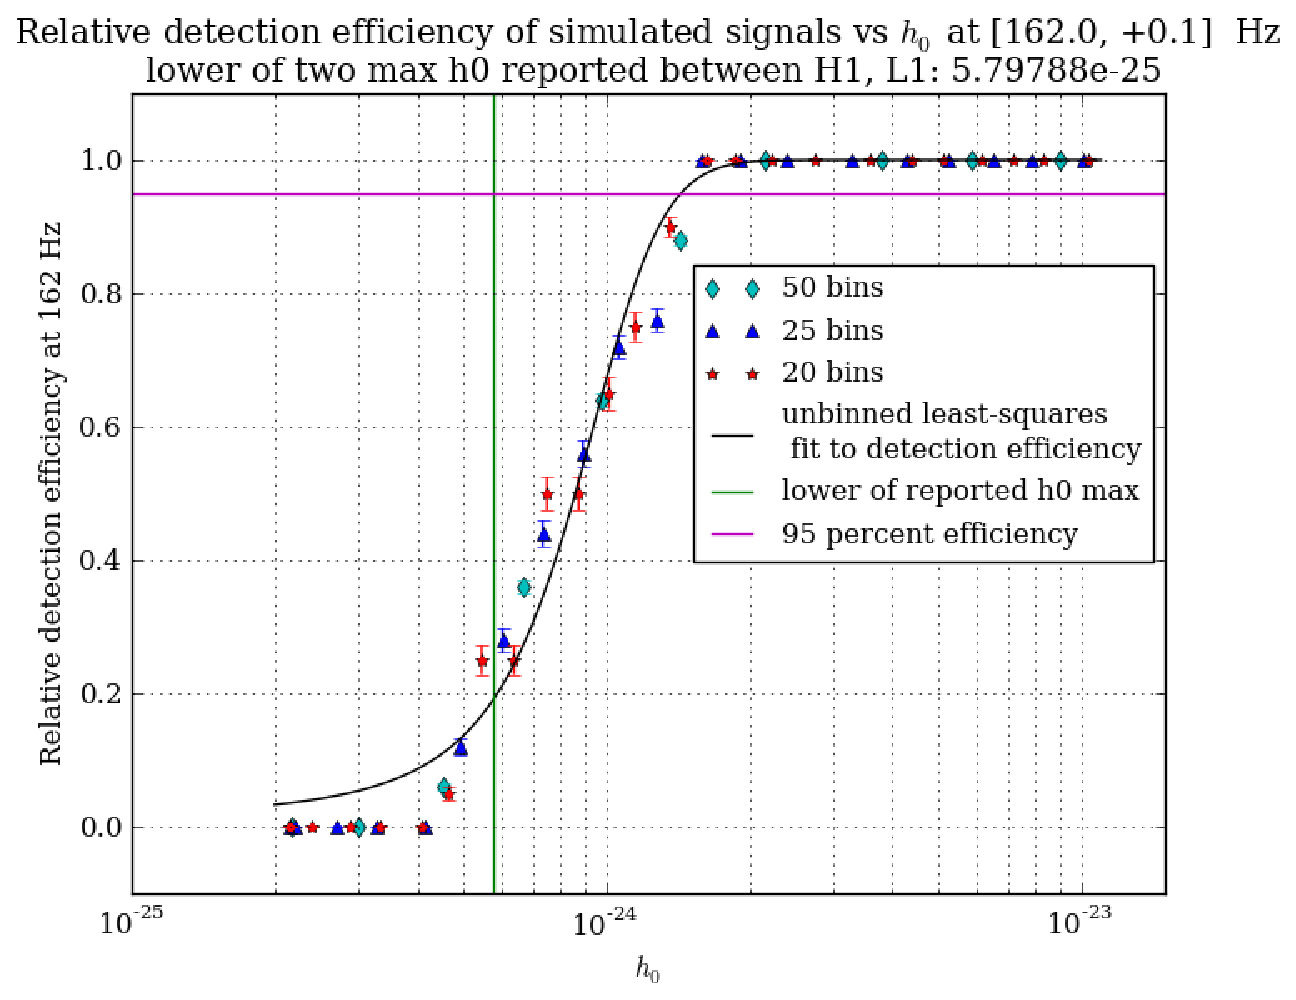
\includegraphics[width=0.70\paperwidth,height=0.48\paperheight]{plots/detectionEfficiencyh0-162-0Hz.eps}
\caption{
Detection efficiency of 500 injections (each at H1, L1) into
S6 data at 162 Hz, given threshold $\log_{10}p = -7.75$}
\label{S6_det_eff_162}
\end{center}
\end{figure}


Figure~\ref{S6_det_eff_162} shows the detection efficiency curve of TwoSpect at 162 Hz, where the noise floor of the interferometers is very similar to that of 142 Hz. 
Results are consistent with Figure~\ref{S6_det_eff_142}.
The sigmoid trace shows the least-squares best fit to the raw data, which is also plotted at several levels of binning.

\subsection{Real S6 data: $h_0$ recovered vs injected}

\begin{figure}
\begin{center}
\includegraphics[width=0.70\paperwidth,height=0.48\paperheight]{plots/h0UL-vs-h0injected-162-0Hz.eps}
\caption{
Raw $h_0$ \& tentative 95\% confidence UL $>2\times10^{-24}$; 500 injections
into S6 data at 162 Hz (injections also done at 142, 222 Hz)}
\label{S6_ULs_162}
\end{center}
\end{figure}


Figure~\ref{S6_ULs_162} correspondingly shows the $h_0$ upper limit versus $h_0$ injected curve of TwoSpect at 162 Hz.
Analogously, it resembles Figure~\ref{S6_ULs_142}.
Note that the lower $h_0$ injected values, on the left side of the plot, return a higher upper limit than their true value.
Injections are recovered more rarely as $h_0$ diminishes, eventually blending into interferometer noise.
One of our concerns has been how non-Gaussian data might affect upper limits, and this figure shows that TwoSpect is again highly robust.
On the right side of the plot, with increasing $h_0$ injected, the recovered upper limit parallels the injection value, with a confidence level multiplier to ensure that the UL is higher than the true value at least 95\% of the time even with arbitrary underlying $\cos \iota$ and uncertain $a \sin i$.

%\subsubsection{Real S6 data: $p$-weighted $h_0$ recovered vs injected}
%\begin{figure}
%\caption{\protect\includegraphics[width=0.5\paperwidth,height=0.35\paperheight]{plots/p-weighted/h0UL-vs-h0injected-162-0Hz.eps}}
%Raw $h_0$, and tentative 95\% confidence UL, for 500 injections into\\
%S6 data at 162 Hz (injections also done at 142, 222 Hz)
%\end{figure}



\section{Real data: detection efficiency at 222 Hz}

\begin{figure}
\begin{center}
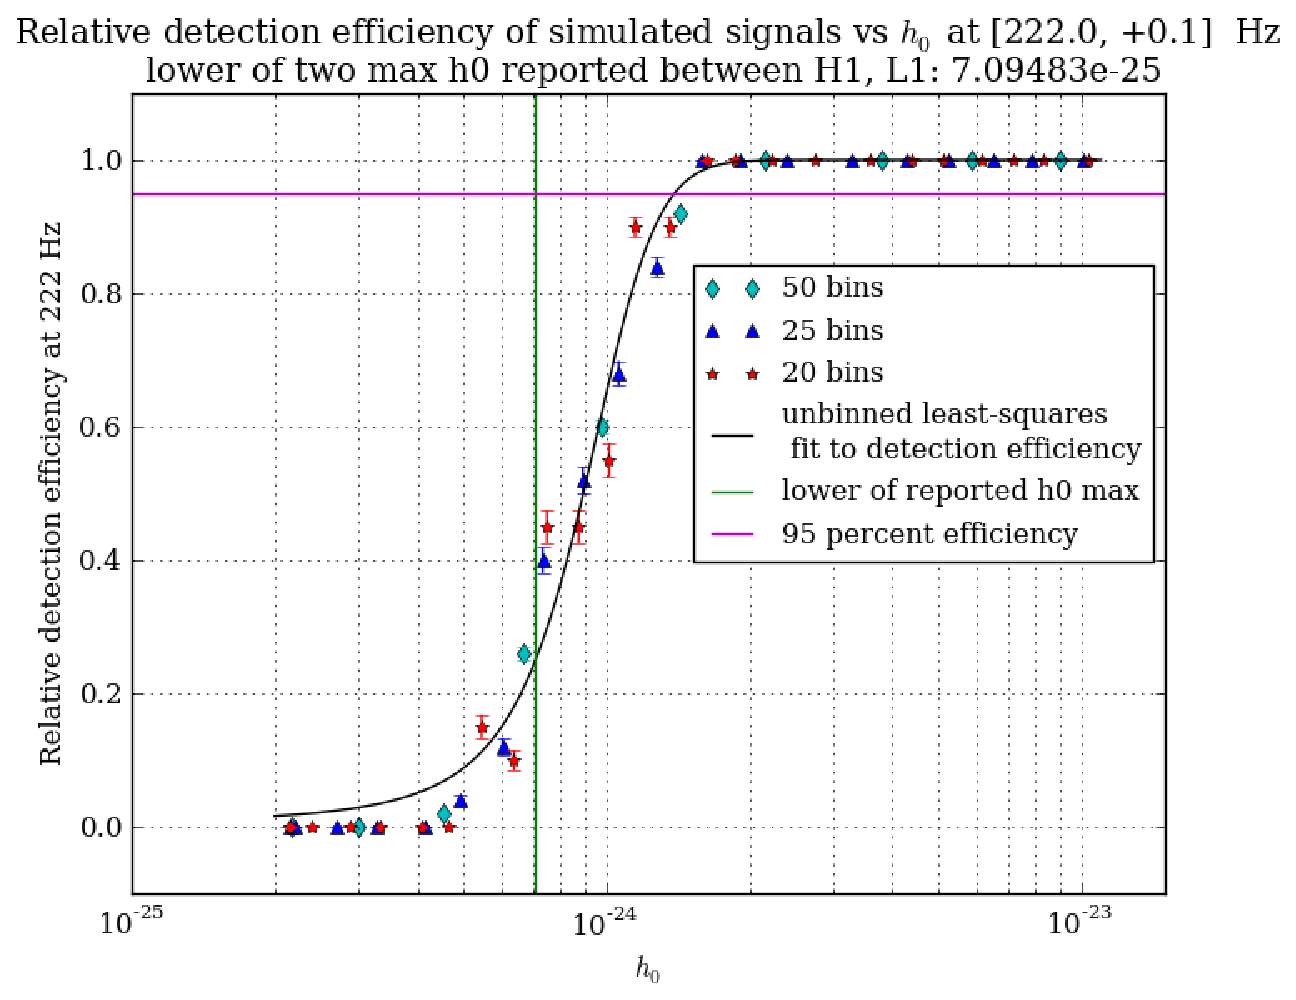
\includegraphics[width=0.70\paperwidth,height=0.48\paperheight]{plots/detectionEfficiencyh0-222-0Hz.eps}
\caption{
Detection efficiency of 500 injections (each at H1, L1) into
S6 data at 222 Hz, given threshold $\log_{10}p = -7.75$}
\label{S6_det_eff_222}
\end{center}
\end{figure}

Just like Figure~\ref{S6_det_eff_162}, Figure~\ref{S6_det_eff_222} shows the detection efficiency curve, albeit in the slightly-higher noise floor at 222 Hz.

\subsection{Real S6 data: $h_0$ recovered vs injected}

\begin{figure}
\begin{center}
\includegraphics[width=0.70\paperwidth,height=0.48\paperheight]{plots/h0UL-vs-h0injected-222-0Hz.eps}
\caption{
Raw $h_0$ \& tentative 95\% confidence UL $>2\times10^{-24}$; 500 injections
into S6 data at 222 Hz (injections also done at 142, 162 Hz)}
\label{S6_ULs_222}
\end{center}
\end{figure}

Injections, as in Figure~\ref{S6_ULs_162}, are shown with recovered upper limits in Figure~\ref{S6_ULs_222}.
TwoSpect successfully recovers injections with the same confidence level factor in each of the three injection bands: 142, 162, and 222 Hz.

%\subsubsection{Real S6 data: $p$-weighted $h_0$ recovered vs injected}
%\begin{figure}
%\caption{\protect\includegraphics[width=0.5\paperwidth,height=0.35\paperheight]{plots/p-weighted/h0UL-vs-h0injected-222-0Hz.eps}}
%Raw $h_0$, and tentative 95\% confidence UL, for 500 injections into\\
%S6 data at 222 Hz (injections also done at 142, 162 Hz)
%\end{figure}


%\subsection{S6: $p$-weighted Sco X-1 upper limits, random polarization}
%\begin{figure}
%\caption{\protect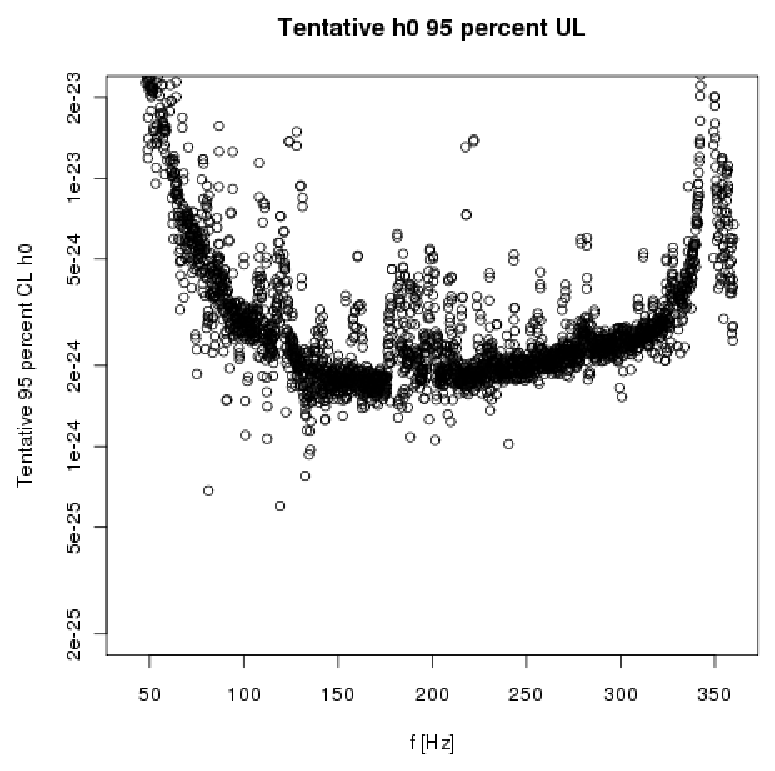
\includegraphics[width=0.5\paperwidth,height=0.35\paperheight]{plots/p-weighted/h0FullUL95logGuess-H1.eps}}
%H1: loudest $h_0 \times \left( 1 + \frac{\log_{10} p}{-7.75} \right) \times \left[\cos \iota \textup{ factor}\right]$ in 0.1 Hz bands
%\end{figure}
%\begin{figure}
%\caption{\protect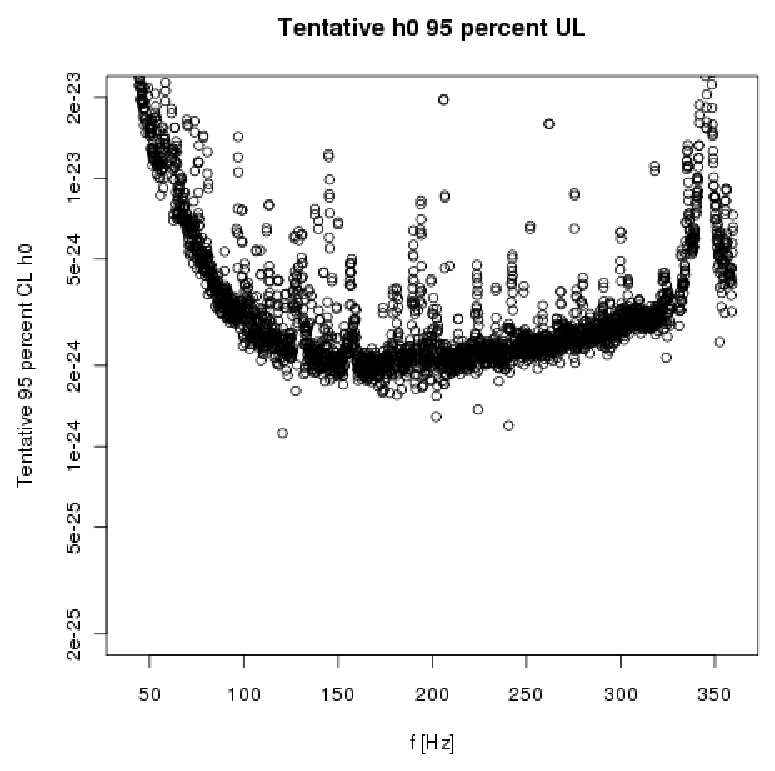
\includegraphics[width=0.5\paperwidth,height=0.35\paperheight]{plots/p-weighted/h0FullUL95logGuess-L1.eps}}
%L1: loudest $h_0 \times \left( 1 + \frac{\log_{10} p}{-7.75} \right) \times \left[\cos \iota \textup{ factor}\right]$ in 0.1 Hz bands
%\end{figure}

\section{S6: Scorpius X-1 upper limits, raw circular output}

\begin{figure}
\begin{center}
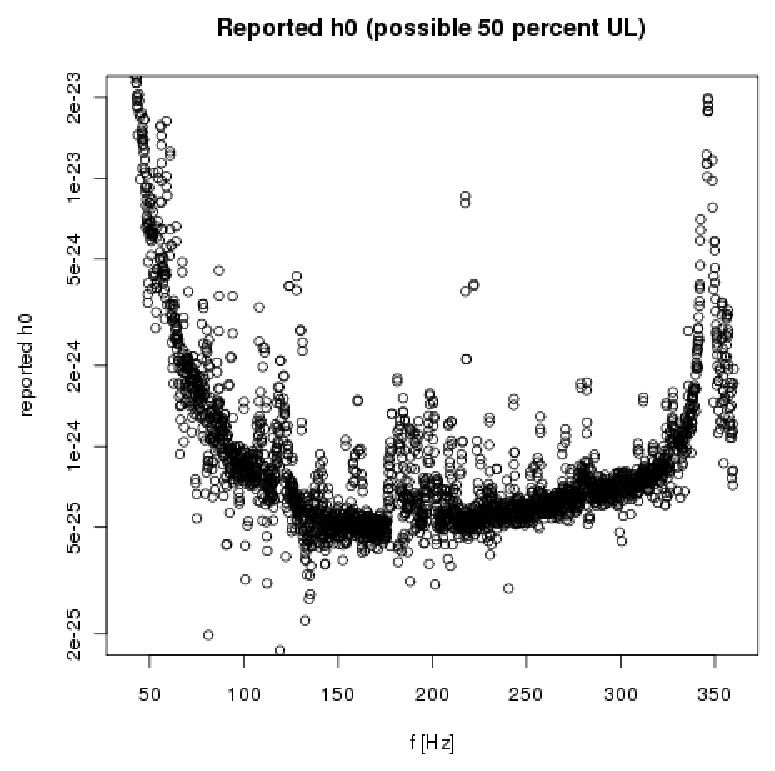
\includegraphics[width=0.68\paperwidth,height=0.48\paperheight]{plots/h0FullUL50log-H1.eps}
\caption{
H1: loudest $h_0$ in 0.1 Hz bands, effectively circular polarization}
\label{S6_H1_raw_output_UL}
\end{center}
\end{figure}

\begin{figure}
\begin{center}
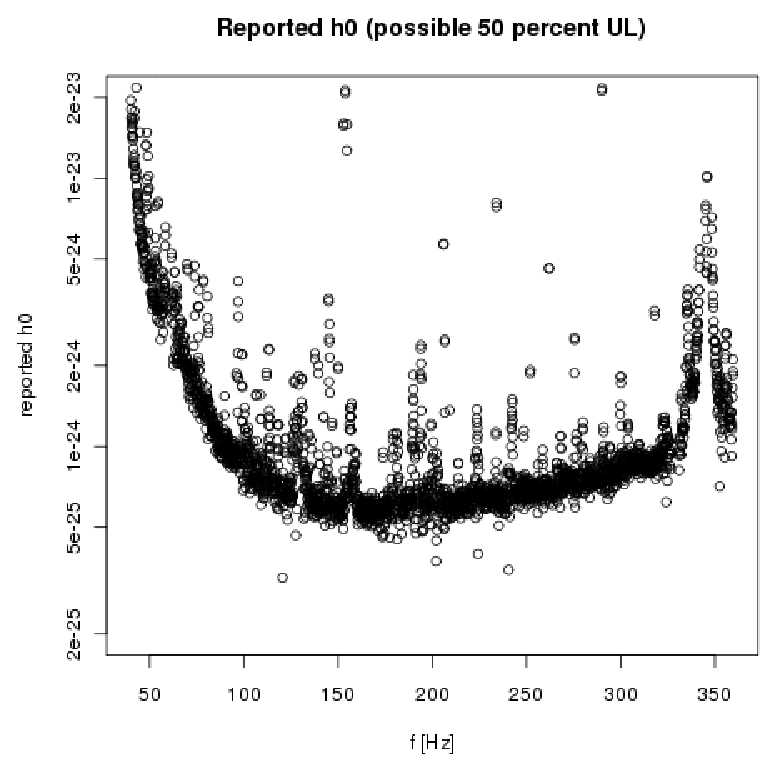
\includegraphics[width=0.68\paperwidth,height=0.48\paperheight]{plots/h0FullUL50log-L1.eps}
\caption{
L1: loudest $h_0$ in 0.1 Hz bands, effectively circular polarization}
\label{S6_L1_raw_output_UL}
\end{center}
\end{figure}

TwoSpect's $h_0$ output, proportional to the $R$ statistic, has been tested and is informative for the all-sky search~\cite{GoetzTwoSpectMethods2011,GoetzTwoSpectResults2014}.
This $h_0$ value corresponds to a circularly polarized gravitational wave.
Without any corrections, the output is seen in Figures~\ref{S6_H1_raw_output_UL} and~\ref{S6_L1_raw_output_UL}.
The confidence level of these values in the multi-trial, directed search over the fully-templated $df$ vs $f$ plane required Figures~\ref{S6_ULs_142}, \ref{S6_ULs_162}, and \ref{S6_ULs_222} to interpret. 
Corrected by Equation~\ref{S6_UL_formula} and taking the lower of either upper limit when a band is covered by both H1 and L1, the joint upper limit is seen in Figure~\ref{S6_H1L1_UL}.
With this knowledge, the author has interpreted the TwoSpect S6 results as a broadband upper limit, from 40 to 2040 Hz, on gravitational wave emission from Scorpius X-1.
